% enable this to activate the version for PRINT
% disable this to make the pdf symmetric and without white pages
% => asymmetric alternating left/right margins
% \newcommand*{\printversion}{}%

%% | ---------------- document meta information --------------- |

\newcommand{\Author}{Jakub Pelc}
\newcommand{\Department}{Department of Cybernetics}
\newcommand{\Supervisor}{Ing. Vojtěch Vrba}
\newcommand{\SupervisorSpecialist}{RNDr. Petr Štěpán, Ph.D.}
\newcommand{\Programme}{Open Informatics}
\newcommand{\Field}{Artificial Intelligence and Computer Science}
\newcommand{\Title}{Relative Pose Estimation Using Event-Based Measurements of LED Signals}
\newcommand{\Keywords}{Unmanned Aerial Vehicles, Event Cameras}
\newcommand{\KlicovaSlova}{Bezpilotní Prostředky, Eventové Kamery}
\newcommand{\Year}{2025}
\newcommand{\Month}{May}
\newcommand{\Date}{\Month~\Year}
\newcommand{\Location}{Prague}

%% | ---------------------- configuration --------------------- |

% most of the configuration stuff happens here
\input{src/document_setup.tex}

%% | ---------------------- the contents ---------------------- |

\begin{document}

% this will prevent unwanted line overflows
% http://latexref.xyz/_005cfussy-_0026-_005csloppy.html
\sloppy

\pagenumbering{roman}

%% --------------------------------------------------------------
%% |                         Title page                         |
%% --------------------------------------------------------------

\input{src/title}

% set up the page style for the "intro" pages
\pagestyle{plain}

%% --------------------------------------------------------------
%% |                       Acknowledgments                      |
%% --------------------------------------------------------------

\conditionalClearPage

\input{src/acknowledgments.tex}

%% --------------------------------------------------------------
%% |                         Assignment                         |
%% --------------------------------------------------------------

\conditionalClearPage

\includepdf{src/assignment.pdf}

%% --------------------------------------------------------------
%% |                         Declaration                        |
%% --------------------------------------------------------------

\conditionalClearPage

\input{src/declaration.tex}

%% --------------------------------------------------------------
%% |                          Abstracts                         |
%% --------------------------------------------------------------

\conditionalClearPage

\input{src/abstract_en.tex}

\conditionalClearPage

\input{src/abstrakt_cz.tex}

%% --------------------------------------------------------------
%% |                        Abbreviations                       |
%% --------------------------------------------------------------

\conditionalClearPage

\begin{changemargin}{0.8cm}{0.8cm}

~\vfill{}

\section*{Abbreviations}

% this will print only the used abbreviations
%!TEX root = ../main.tex

\begin{acronym}
  \acro{API}[API]{Application Programming Interface}
  \acro{CTU}[CTU]{Czech Technical University}
  \acro{DOF}[DOF]{degree-of-freedom}
  \acro{FOV}[FOV]{Field of View}
  \acro{GNSS}[GNSS]{Global Navigation Satellite System}
  \acro{GPS}[GPS]{Global Positioning System}
  \acro{IMU}[IMU]{Inertial Measurement Unit}
  \acro{LED}[LED]{Light Emitting Diode}
  \acro{LKF}[LKF]{Linear Kalman Filter}
  \acro{LTI}[LTI]{Linear time-invariant}
  \acro{LiDAR}[LiDAR]{Light Detection and Ranging}
  \acro{MAV}[MAV]{Micro Aerial Vehicle}
  \acro{MPC}[MPC]{Model Predictive Control}
  \acro{MRS}[MRS]{Multi-robot Systems Group}
  \acro{ROI}[ROI]{Region of Interest}
  \acro{ROS}[ROS]{Robot Operating System}
  \acro{RSSR}[RSSR]{Received Signal Strength Ratio}
  \acro{RTK}[RTK]{Real-time Kinematics}
  \acro{SLAM}[SLAM]{Simultaneous Localization And Mapping}
  \acro{UAV}[UAV]{Unmanned Aerial Vehicle}
  \acro{UGV}[UGV]{Unmanned Ground Vehicle}
  \acro{UKF}[UKF]{Unscented Kalman Filter}
  \acro{VLP}[VLP]{Visible Light Positioning}
\end{acronym}


\vskip 2.5cm

\end{changemargin}

\conditionalClearPage

%% --------------------------------------------------------------
%% |                      Table of contents                     |
%% --------------------------------------------------------------

\tableofcontents

\conditionalClearPage

% set up the full page style with normal page numbering
\pagestyle{full}
\pagenumbering{arabic}

%% --------------------------------------------------------------
%% |            introduction (and working principles)           |
%% --------------------------------------------------------------

%!TEX root = ../main.tex

\chapter{Introduction\label{chap:introduction}}

This semestral project is focused on measuring the influence of distance and frequency of modulated
light source on event based camera response. Knowing the parameters of the light source, the camera with the lens
and how the response behaves, it is possible to predict the distance of the light source from the camera. This can be
used to improve the precision of localization algorithms, that are used in \ac{UAV} swarming applications. 

Event based cameras, in contrast to traditional frame based cameras, do not capture still frames but rather
provide an asynchronous and idependent stream of intensity changes on individual pixels.
Each pixel memorizes the last intensity value and sends an event when the intensity changes above a certain threshold.
%\cite{gallego2020event}
Event cameras circumvent many common issues found in traditional frame-based cameras, such as motion blur caused
by fast-moving objects. They offer significant advantages, including a high dynamic range, low latency,
and energy efficiency.
This makes them perfect fot the application of agile robotics,
where the fast response time is crucial (especially in UAV swarming situations). With their sub-millisecond response time,
event cameras can provide a significant advantage over traditional cameras in these applications.
However, they also come with some drawbacks, such as the need for a different approach to
data processing and the higher cost of the camera units themselves. \cite{gallego2020event}

The event data stream is represented by tuples of $(x, y, p, t)$, where $(x, y)$ are the pixel coordinates, $t$ is the time of
intensity change and $p$ is the polarity of the change - the increase or decrease of light intensity. Images can be
reconstructed from the event stream by integrating the events over time, doing so makes the usage of normal vision 
algorithms is possible, but is also goes against the main advantage of the event cameras - the low latency.

\section{Related Works}

The unique capabilities of event-based cameras have been extensively explored in various applications and studies.
A comprehensive survey by Gallego et al. highlights the advantages of event cameras in
applications requiring high-speed motion analysis, wide dynamic range, and low power consumption. \cite{gallego2020event}
%The survey also addresses the challenges of processing the asynchronous and sparse event data these cameras generate, 
%emphasizing the need for novel algorithms tailored to this unconventional sensing paradigm.

The potential of event cameras in vehicular \ac{VLC} has been demonstrated by Shen et al.
Their study introduced a framework utilizing a \ac{DVS} to mitigate the limitations of
traditional photodiode- and frame-based camera systems, such as limited throughput and vulnerability to ambient
interference. By leveraging the event-driven nature of DVS, the proposed system achieved significant improvements
in data transmission range and robustness. \cite{shen2019vehicular}

% In addition to VLC, event-based cameras have been successfully integrated into localization systems,
% yielding promising results for indoor positioning. Jung et al. introduced an indoor positioning method based on the
% \ac{RSSR} using LEDs for location estimation. This approach leverages the relative ratio of optical power detected by
% photodiodes from multiple LED sources, achieving precise positioning with a mean error of 3.24 cm. By incorporating
% time-division multiplexing, the method ensures robust identification of individual LEDs, enabling efficient localization.
% This system highlights potential applications in autonomous navigation and UAV swarming, benefiting from the method's high
% accuracy and low additional infrastructure requirements \cite{jung2014rssr}.

Event-based cameras have been integrated into localization systems with promising indoor positioning results.
Jung et al. demonstrated an \ac{RSSR}-based method using LEDs and time-division multiplexing, achieving precise positioning
with a mean error of 3.24 cm and minimal infrastructure requirements, suitable for applications like autonomous navigation
and UAV swarming \cite{jung2014rssr}.

%% --------------------------------------------------------------
%% |                   Event camera response                    |
%% --------------------------------------------------------------

%!TEX root = ../main.tex

\chapter{Response of an event-based camera\label{chap:response}}

\section{Equipment}

The event based camera used in this work is the model EVK4\footnote{Prophesee EVK4 website: \url{https://www.prophesee.ai/event-camera-evk4/}.}, manufactured by Prophesee. The camera has a resolution of 
$1280 \times 720$ pixels, with maximum frame rate equivalent of 10k fps and a dynamic range of 120 dB.
A fish eye lens with an inbuilt UV filter was used during the measurements to target the specific wavelength of the LEDs
that are used on the UAVs. The UAV used for measurements was a unit from the MRS UVDAR system, with UV \ac{LED} light sources, mounted at each arm of the UAV, which are used for localization and communication purposes.
Both can be seen on \reffig{fig:uavcam}.

\begin{figure}[H]
	\centering
	\subfloat[The event-based camera EVK4 from Prophesee with a fish eye lens.] {
	  \includegraphics[width=0.5\textwidth]{./fig/photos/evk4.jpg}
	  \label{fig:evk4}
	}
	\subfloat[MRS UVDAR UAV unit] {
	  \includegraphics[width=0.5\textwidth]{./fig/photos/uav1.jpeg}
	  \label{fig:uav1}
	}
	\caption{
  An event-based camera with a fish eye lens can be seen on \reffig{fig:evk4}, which was used to measure the UV LEDs mounted on the UAV unit from the MRS UVDAR system as seen on \reffig{fig:uav1}.
  }
	\label{fig:uavcam}
\end{figure}

The data from the camera has been obtained using the Metavision Studio software, which records the data in the \texttt{.raw} format.
Data is then later processed using various functions from the Metavision SDK\footnote{Metavision SDK Docs: \url{https://docs.prophesee.ai/stable/index.html}},
which has either C++ or Python API. In this work, the Python API has been used.

\section{Data collection}

The data has been collected on several occasions by measuring a stationary UAV at various distances and rotations from the camera.
Each UAV is equipped with 8 UV LEDs, with 2 LEDs on each arm of the UAV. Each of the LEDs can be individually controlled
and can be set to various sequences of blinking, and a common modulation frequency can be set for all LEDs.

\subsection{Initial measurements}

The initial measurements were done by securing the event camera on a tripod and placing the UAV at distances ranging from
$0.5$ to $2.5$ meters. The LEDs were set to blink at a frequency in range from $1$ Hz to $30$ kHz. No \ac{ROI} was set
and the whole visible area has been recorded during the testing.

This first experiment proved to be rather inefficient, as the LEDs need to be isolated from each other's influence, which
was not done properly at this time. This problem is solvable in the post processing, by filtering out the events
by using a ROI filter (it is possible to filter the events by finding bounding boxes
that encapsulate light sources, but on a more complex scene this approach becomes relatively hard).
The other issue turned out to be the reflections of surrounding objects (as seen on \reffig{fig:meas1}), which caused
another source of unwanted events in the recording, which may in turn confuse some blob detection methods.

\begin{figure}[H]
	\centering
	\subfloat[An event-camera view of the UAV with UV LEDs.] {
	  \includegraphics[width=0.5\textwidth]{./fig/photos/meas1.png}
	  \label{fig:meas1_e}
	}
	\subfloat[View of the experiment setup.] {
	  \includegraphics[width=0.5\textwidth]{./fig/photos/meas1_c.png}
	  \label{fig:meas1_c}
	}
	\caption{
  The setup for measuring the event-camera response with a EVK4 camera. Visible reflections from a wall can be seen on \reffig{fig:meas1}. The setup is shown on \reffig{fig:meas1_c}.
  }
	\label{fig:meas1}
\end{figure}


\subsection{Distance - frequency influence}

In the following measurements, we consider only one source of light as the whole ending of the arm of the UAV (with 2 UV LEDs). Other arm light sources were turned off during the measurements.
Measurements were done on areas isolated by ROI filter directly in Metavision Studio, events were collected only on one select area around the light source, with the
rest of the events being discarded.
This time, the position of the UAV was fixed relative to the camera on a blank background. The camera was placed on a tripod
and moved by increments of $0.2$ meters, starting from $1$ meter and ending at $3$ meters, with additional measurements done
at $4$ and $5$ meters.
Frequency range of the LED modulation was set in a range from $10$ Hz to $30$ kHz, with blinking sequence set to \texttt{0, 1}.

\subsection{Rotation angle influence}

In addition to distance and frequency influence, the rotation angle influence also needs to be considered, to
verify the emitting characteristics of the light sources - if they can or cannot be considered lambertian.
The UAV was rotated by increments of $45$ degrees relative to the event camera, at distances of $0.5$, $1$ and $2$ meters,
with frequencies ranging from $10$ Hz to $10$ kHz and the blinking sequence was set to \texttt{0, 1}.

\subsection{RSSR Data collection}

Another dataset was collected for the application of \ac{RSSR} \cite{sooyongrssr}, which we analyze more in \refchap{chap:rssr}.
The data includes calibration data, that is necessary for the optical system parameter estimation. This calibration is done by
recording a video using a calibration lattice of LEDs with known spacing, and observing the pattern distortion in the
resulting video.
The UAV was placed at increasing distances and various angles relative to the event camera, with the LEDs blinking at frequencies different from
each other. 
The blinking sequences were set to the following values:
\begin{lstlisting}
	led_1 = [0, 0, 0, 0, 0, 0, 0, 0, 1, 1, 1, 1, 1, 1, 1, 1]
	led_2 = [0, 0, 0, 0, 1, 1, 1, 1, 0, 0, 0, 0, 1, 1, 1, 1]
	led_3 = [0, 0, 1, 1, 0, 0, 1, 1, 0, 0, 1, 1, 0, 0, 1, 1]
	led_4 = [0, 1, 0, 1, 0, 1, 0, 1, 0, 1, 0, 1, 0, 1, 0, 1]
\end{lstlisting}
with a common modulation frequency of $250$ Hz.
This allows for the measurement of the ratio
%explain why to use the ratio, not the absolute value
\footnote{Using the absolute value of the LED power is not suitable, as it also depends of the camera settings, surrounding
environment and other factors. Finding such ratio (or property) that stays constant is crucial for correct distance estimation.}
between the responses for each of the LEDs, which is necessary
for the estimation of the UAV position using RSSR.

\section{Event response data processing}

The event-camera response data has ben analyzed using Python in a Jupyter notebook
\footnote{Source code is available at: \url{https://github.com/kubakubakuba/mrs-uvdar-distance-estimator/blob/main/main.ipynb}},
with libraries from Metavision SDK\footnote{Metavision SDK Docs: \url{https://docs.prophesee.ai/stable/index.html}}.
The notebook is divided into sections that represent several datasets that were recorded during the measurements.
Precomputed average number of events with the standard deviation is stored in \texttt{.npz} files in the \texttt{./data} directory to speed up the visualization process.

\subsection{Distance - frequency influence}

The distance frequency dataset has recordings of the UAV placed at 0 and 45 degrees relative to the event camera. This ensures data is captured from either
one LED source pointed directly at the event camera, or 2 LED sources pointed at the event camera at an angle. At each distance a new subdirectory was
created, with its name being the distance in meters and the content being the recordings of various frequencies in sequence, ordered by the recording timetamp.
With the range of frequencies\footnote{The frequencies represented in this list are the actual frequencies sent to the UVDAR unit. The preserved frequencies
are half of the values in this list - UVDAR interprets the frequency with a reference to the length of the sequence (here the sequence being \texttt{0, 1}).} and distances being
\begin{lstlisting}
frequencies_Hz = [10, 25, 50, 100, 250, 500, 1000, 2500, 5000, 10000, 20000, 30000]
distances_m = [1.0, 1.2, 1.4, 1.6, 1.8, 2.0, 2.2, 2.4, 2.6, 2.8, 3.0, 4.0, 5.0]
\end{lstlisting}
We can load the dataset stored in raw files into a matrix representing the distances and frequencies, then load a select amount of events from each file.
The data is then resampled into a 1D array by summing polarities over a select bin width
\footnote{The bin width should be adjusted appropriately, as the farther the event camera is from the source, the fewer events are generated.}.
Peaks in this signal are then analyzed by SciPy's \texttt{findpeaks} function,
and the average amount of events with the standard deviation is calculated for each frequency and distance.

We can see the influence of distance and frequency on the average number of events on
\reffig{fig:dist} and \reffig{fig:freqs} respectively. The data shows a decreasing trend of the average number of events
with the increase of distance or frequency. The drop related to the distance can be explained by the perceived intensity
decrease of the light source with an increasing distance. With an increasing frequency, the camera is not able to capture
all the changes that are generated by the light source. On very high frequencies and distances, the camera is not able
to detect any real events at all, as there is more noise generated by the camera itself at this point. This can be observed
at \reffig{fig:dist_2} with the frequency of $30$ kHz at $3$ meters.

If we now select one frequency and try to fit it with a curve,
we can see that the data can be approximated with a rational or exponential function as shown on \reffig{fig:fit1}.
The best fit without being too complex is the inverse square law, which can be expressed as
\begin{equation}
	\text{intensity} \propto \frac{1}{\text{distance}^2}
\end{equation}

\begin{figure}[H]
	\centering
	\subfloat[Influence of distance on the average number of events.] {
	  \includegraphics[width=0.5\textwidth]{./fig/semestral/dist.pdf}
	  \label{fig:dist_1}
	}
	\subfloat[Influence of distance on the log of average number of events.] {
	  \includegraphics[width=0.5\textwidth]{./fig/semestral/distlog.pdf}
	  \label{fig:dist_2}
	}
	\caption{
  The influence of distance on the average number of events with the UAV rotated 0 degrees relative to the event camera on \reffig{fig:dist_1}, and with the log of the average number of events on \reffig{fig:dist_2}.
  }
	\label{fig:dist}
\end{figure}
\begin{figure}[H]
	\centering
	\subfloat[Influence of frequency on the average number of events.] {
	  \includegraphics[width=0.5\textwidth]{./fig/semestral/freq.pdf}
	  \label{fig:freqs_1}
	}
	\subfloat[Influence of frequency on the log of average number of events.] {
	  \includegraphics[width=0.5\textwidth]{./fig/semestral/freqlog.pdf}
	  \label{fig:freqs_2}
	}
	\caption{
  The influence of frequency on the average number of events with the UAV rotated 0 degrees relative to the event camera on \reffig{fig:freqs_1}, and with the log of the average number of events on \reffig{fig:freqs_2}.
  }
	\label{fig:freqs}
\end{figure}

\begin{figure}[H]
	\centering
	\includegraphics[width=0.90\textwidth]{./fig/semestral/inverse_square/square.pdf}
	\caption{Influence of distance data fitted with various curves.}
	\label{fig:fit1}
\end{figure}
More complex functions could be used to fit the data, but they would likely lead to overfitting rather than capturing the underlying trend in a generalizable way.
The inverse square law provides a relatively good approximation of the data.

\subsection{Rotation angle influence}
From the manufacturers datasheet for the UV LEDs\footnote{The datasheet of ProLight PM2B-1LLE 1W UV Power LED can be obtained from \url{https://www.tme.eu/Document/9dfb498784ffdd07892a42f4f17c6f37/PM2B-1LLE-DTE.pdf}}
used in the UVDAR system, we can learn that the LEDs have a lambertian radiation pattern,
which can be seen on \reffig{fig:lambertian}.
\begin {figure}[H]
	\centering
	\includegraphics[width=0.75\textwidth]{./fig/semestral/lambertian/lambertian.pdf}
	\caption{Lambertian radiation pattern of the UV LED.}
	\label{fig:lambertian}
\end{figure}

This means that the intensity of the light emmited from the LED decreases with the cosine
of the angle between the normal of the LED and the direction of the light \refeq{eq:lambertian}.
\begin{equation}
	I(\theta) = I_0\cos(\theta)
	\label{eq:lambertian}
\end{equation}
If we shift those distributions by $\pm 45$ degrees and sum them together, we can see the
theoretical distribution of the light emmited from the singular UAV arm \reffig{fig:lambert_combined}.
\begin {figure}[H]
	\centering
	\includegraphics[width=0.50\textwidth]{./fig/semestral/lambertian/3lambertian.pdf}
	\caption{Radiation pattern of two lambertian light sources shifted by $\pm 45$ degrees.}
	\label{fig:lambert_combined}
\end{figure}
With the dataset of the rotation of the UAV relative to the camera we will get the following results
on \reffig{fig:angles}.

\begin{figure}[H]
	\centering
	\subfloat[Influence of rotation of the UAV on the log of average number of events at 0.5 m.] {
	  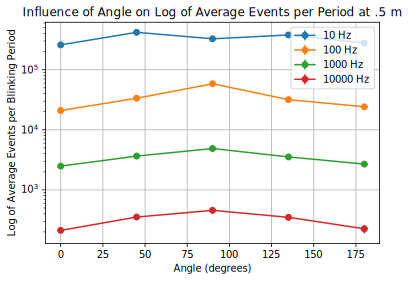
\includegraphics[width=0.5\textwidth]{./fig/semestral/angle1.pdf}
	  \label{fig:angle_1}
	}
	% \subfloat[Influence of rotation of the UAV on the log of average number of events at 1 m.] {
	%   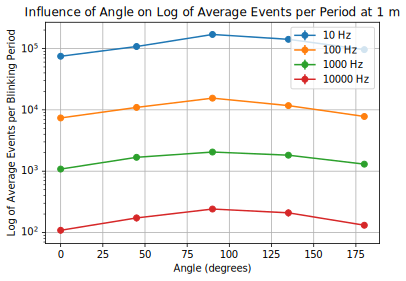
\includegraphics[width=0.5\textwidth]{./fig/semestral/angle2.pdf}
	%   \label{fig:angle_2}
	% }
	\subfloat[Influence of rotation of the UAV on the log of average number of events at 2 m.] {
	  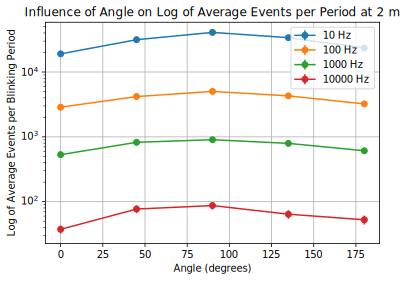
\includegraphics[width=0.5\textwidth]{./fig/semestral/angle3.pdf}
	  \label{fig:angle_3}
	}
	\caption{
  The influence of rotation angle on the log of average number of events at 0.5 m on \reffig{fig:angle_1} and at 2 m on \reffig{fig:angle_3}.
  }
	\label{fig:angles}
\end{figure}
The data shows a rough approximation of the theoretical distribution on \reffig{fig:lambert_combined},
but with a drop of intensity at the middle of the distribution. This could be caused
by the fact that the LEDs, when close to the camera, can be perceived as multiple light sources,
but when moved further away, they merge into one source as shown on \reffig{fig:leds}.

\begin{figure}[H]
	\centering
	\subfloat[2 LEDs with blinking frequency of 10 Hz at 0.5 m.] {
	  \includegraphics[width=0.5\textwidth]{./fig/photos/2leds_05m.png}
	  \label{fig:leds_1}
	}
	\subfloat[2 LEDs with blinking frequency of 10 Hz at 2 m.] {
	  \includegraphics[width=0.5\textwidth]{./fig/photos/2leds_2m.png}
	  \label{fig:leds_2}
	}
	\caption{
  The light source on one arm of the UAV, consisting of two UV LEDs, blinking at a frequency of 10 Hz,
  placed at 0.5 m on \reffig{fig:leds_1} and 2 m at \reffig{fig:leds_2}.
  }
	\label{fig:leds}
\end{figure}
What we can also observe from \reffig{fig:leds} are the star-like shapes of the LEDs, which are supposed to be circular.
Those shapes are caused by light diffraction (and are named diffraction spikes), which is in turn caused by the aperture
blades in the lens of the camera. The number
of star spikes depend on the number of blades, the set aperture and the light source intensity then causes stars of different
levels of profoundness.\cite{lendermann2018computational} We can observe this by comparing how profound the star shapes are on different
frequencies, as shown on \reffig{fig:stars}.

\begin{figure}[H]
	\centering
	\subfloat[LED blinking at 10 Hz at 1.0 m] {
	  \includegraphics[width=0.5\textwidth]{./fig/photos/led_10hz.png}
	  \label{fig:stars_1}
	}
	\subfloat[LED blinking at 1 kHz at 1.0 m] {
	  \includegraphics[width=0.5\textwidth]{./fig/photos/led_1000hz.png}
	  \label{fig:stars_2}
	}
	\caption{
  Two same LED light sources at 1.0 meters, blinking at 10 Hz and 1 kHz.
  \reffig{fig:stars_1} shows a visible diffraction star (while being much brighter), while \reffig{fig:stars_2} shows a
  much more cicular source of light that is not as bright.
  }
	\label{fig:stars}
\end{figure}

%% --------------------------------------------------------------
%% |                   Relative pose estimation                 |
%% --------------------------------------------------------------

%!TEX root = ../main.tex

\chapter{Camera calibration\label{chap:calib}}

As for the correct representation of distances and angles in the received data from the camera, a camera calibration needs to be performed.
The lens used when obtaining the data is a 2.5mm, f/1.6 fish-eye lens, with FOV of more than 90 degrees, which can be seen in \reffig{fig:fisheye_lens}.
\begin{figure}[H]
  \centering
  \includegraphics[width=0.5\textwidth]{./fig/photos/lens.jpeg}
  \caption{2.5mm f/1.6 fish eye lens.}
  \label{fig:fisheye_lens}
\end{figure}
In this work a calibration method proposed by Scaramuzza et al. \cite{scaramuzzacalibration} is used, which is based on the pinhole camera model, and is
used to calibrate fish eye lenses. The implementation used for the calibration is a python library py-OCamCalib \footnote{py-OCamCalib is available at \url{https://github.com/jakarto3d/py-OCamCalib}}.%TODO: maybe cite the github repo
For calibration purposes, a calibration chessboard pattern is usually used, which offers high contrast between squares (and thus easy detections of square corners) and
a known square size. Multiple images are usually taken, at various rotations and distances, to obtain good calibration results.
In our calibration procedure, we use a 5x7 lattice of UV LEDs, which are spaced 50 mm apart from each other. With this pattern, events are generated at the center of the
LEDs, and can be detected by any kind of blob detector. The LED lattice is used, so the event camera can easily detect the events from the bright LEDs, as opposed to
the light being reflected from the chessboard pattern (which does not produce any light on its own).
The calibration lattice can be seen in \reffig{fig:lattice}.

\begin{figure}[H]
	\centering
	\subfloat[Calibration lattice] {
	  \includegraphics[width=0.5\textwidth]{./fig/photos/lattice.jpeg}
	  \label{fig:lattice_1}
	}
	\subfloat[Image from the event camera of the calibration lattice] {
	  \includegraphics[width=0.5\textwidth]{./fig/photos/lattice_evs.png}
	  \label{fig:lattice_2}
	}
	\caption{
		Calibration lattice of 5x7 UV LEDs on \reffig{fig:lattice_1} and the events being produced when placed in front of the camera at \reffig{fig:lattice_2},
		with typical fish-eye lens distortion.
  }
	\label{fig:lattice}
\end{figure}
The downside of using an LED lattice instead of a chessboard pattern, is that at a very high FOV, the distortion of the fish eye lens sometimes does not allow
reliable detection of the exact blob centers (or which events correspond to which LED), as can be seen at \reffig{fig:calibration_pattern_distorted}.
\begin{figure}[H]
  \centering
  \includegraphics[width=0.7\textwidth]{./fig/photos/lattice_280.png}
  \caption{Calibration pattern with 5x7 lattice of UV LEDs, taken with a lens with FOV of 280 degrees.}
  \label{fig:calibration_pattern_distorted}
\end{figure}

As we are not using a regular image of a chessboard pattern, rather a recording of accumulated events, some data preprocessing has to be done beforehand.
For the purpose of this a simple Python app has been written. An event raw recording is loaded, and events are accumulated over a select period of time.
The accumulated events are then saved to a grayscale image, where each pixel corresponds to the number of events that occured at that
pixel \footnote{\url{https://github.com/kubakubakuba/metavision-pyocamcalib/blob/main/generate_frames.py}}. The image is then normalized,
and the LED centers are detected using \texttt{findContours} function from OpenCV \footnote{\url{https://github.com/kubakubakuba/metavision-pyocamcalib/blob/main/detect_blob_centers.py}}.
The detected centers can be then manually labeled (with optional corrections) row-wise, so the calibration script can then perform the calibration.
After this, the regular calibration script from py-OCamCalib can be used. The labeling of the LED centers can be seen in \reffig{fig:calibration_pattern_labeled}.

\begin{figure}[H]
  \centering
  \includegraphics[width=0.7\textwidth]{./fig/photos/lattice_blobs.png}
  \caption{Calibration pattern with 5x7 lattice of UV LEDs, with the centers of the LEDs being labeled.}
  \label{fig:calibration_pattern_labeled}
\end{figure}

After the calibration we are able to map the 3D world coordinates to the 2D image plane. For this, the calibration method needs to obtain the extrinsic
and intrinsic parameters of the camera, where the extrinsic parameters are the rotation and translation of the camera with respect to the world frame, and can be expressed
by equation \ref{eq:extrinsic}.
\begin{equation}
	\begin{bmatrix}
		X_{camera} \\
		Y_{camera} \\
		Z_{camera}
	\end{bmatrix}
	= R 
  \begin{bmatrix}
	X_{world} \\
	Y_{world} \\
	Z_{world}
  \end{bmatrix}
  + T
  \label{eq:extrinsic}
\end{equation}
which is an affine transformation that uses a rotation matrix $R$ and a translation vector $T$. The origin of the camera's coordinate system is at the optical center,
that is at the intersection of the optical axis from the center of the image with the image plane. This can be represented by \reffig{fig:camera_extrinsic}.

\begin{figure}[H]
  \centering
  \includegraphics[width=0.7\textwidth]{./fig/tikz/extrinsic.pdf}
  \caption{Extrinsic parameters of the camera.}
  \label{fig:camera_extrinsic}
\end{figure}

Next step in the camera calibration is to fit an encompassing ellipse to the received data. The purpose of this is to see the fish eye lens distortion center, as well
as the stretching of the image in both the x and y axis. This process can be seen in \reffig{fig:ellipse}. This ellipse is then used to calculate the point mapping functions, which allows for tranformation of points from
the image plane to their respective 3D coordinates.

\begin{figure}[H]
	\centering
	\includegraphics[width=0.9\textwidth]{./fig/tikz/ellipse.pdf}
	\caption{}
	\label{fig:ellipse}
  \end{figure}

The intrinsic parameters of the camera specify the image format itself (influenced by the focal length, sensor size and optical center). As there are many mapping
functions that can be used while modelling the lens (their precision is limited by the manufacturing process), Scaramuzza et al. \cite{scaramuzzacalibration} proposed
to fit a polynomial to find the optimal model for the lens calibration. The mapping functions are shown in \reffig{fig:mapping_functions}.
\begin{figure}[H]
  \centering
  \includegraphics[width=0.9\textwidth]{./fig/tikz/mapping.pdf}
  \caption{Fisheye mapping functions, $f$ is a parameter (focal length).}
  \label{fig:mapping_functions}
\end{figure}

After we fit a polynomial, we can map image points into their corresponding 3D vectors by an equation \ref{eq:intrinsic}.
\begin{equation}
	\lambda \cdot \alpha \cdot
	\begin{bmatrix}
		u' \\
		v' \\
		a_0 + a_1 \rho + \dots + a_{N} \rho^{N} 
	\end{bmatrix}
	= \mathbf{P} \cdot \mathbf{X_w} = %TODO: DOUBLE CHECK X_w is really the world point 
	\begin{bmatrix}
		X_c \\
		Y_c \\
		Z_c
	\end{bmatrix}
	\label{eq:intrinsic}
\end{equation}
where:

$\lambda$ is a scalar factor

$\alpha$ is a scaling factor that we obtain from \reffig{fig:ellipse} by stretching the ellipse back to a circle and performing
the affine transformation, $\alpha, \lambda > 0$ 

$\rho$ is the Euclidean distance of a point from the center $\rho = \sqrt{u^2 + v^2}$

$a_0, \dots a_N$ are the coefficients of the polynomial, and $\mathbf{P}$ is 
the perspective projection matrix.

We can also write another relation between a point $\textbf{m}' = \begin{bmatrix} u' & v' \end{bmatrix}^{T}$ on the image plane
and its corresponding point on the sensor plane $\textbf{m} = \begin{bmatrix} u & v \end{bmatrix}^{T}$. The coordinates of 
$\textbf{m}'$ have the origin at the top left corner of the image, whereas the coordinates of $\textbf{m}$ have origin at the image center.
This can be represented by an affine transformation $\textbf{m}' = \textbf{Am} + \textbf{O}_c$, on \ref{eq:affine} \cite{URBAN201572}.

\begin{equation}
	\begin{bmatrix}
		u' \\
		v'
	\end{bmatrix}
	= 
	\begin{bmatrix}
		c & d \\
		e & 1
	\end{bmatrix}
	\begin{bmatrix}
		u \\
		v
	\end{bmatrix}
	+
	\begin{bmatrix}
		o_u \\
		o_v
	\end{bmatrix}
\label{eq:affine}
\end{equation}

where the matrix A accounts for lens-sensor misalignment, and the vector $\textbf{O}_c$ captures the relation with the center of the distortion. 

\section{Calibration results}

The camera calibration was performed on a series of images, where the calibration lattice was placed as various angles and distances from the camera.
For ideal calibration results, the lattice should be placed in all visible parts of the image, as the distortion of the fish eye is more pronounced at the edges
of the visible area. The calibration was performed on a polynomial of degree 4, more would lead to overfitting and is not necessary.
The calibration results can be seen in \reffig{fig:calib_r}.

\begin{figure}[H]
	\centering
	\subfloat[Calibrated lens model function] {
	  \includegraphics[width=0.5\textwidth]{./fig/pgfplot/evk4_projection.pdf}
	  \label{fig:calib_r_1}
	}
	\subfloat[Calibration images mean reprojection errors] {
	  \includegraphics[width=0.5\textwidth]{./fig/pgfplot/evk4_reprojection_error.pdf}
	  \label{fig:calib_r_2}
	}
	\caption{
		Calibration results with the calibrated lens model function highlighted in red in \reffig{fig:calib_r_1} and the calibration images mean reprojection errors on \reffig{fig:calib_r_2}.
  }
	\label{fig:calib_r}
\end{figure}

We can now fit the encompassing ellipse to the data, by minimizing the number of events that are out of the ellipse (minimizing the ellipse size while keeping the
captured events inside). The ellipse can be seen in \reffig{fig:ellipse_fit}.

\begin{figure}[H]
	\centering
	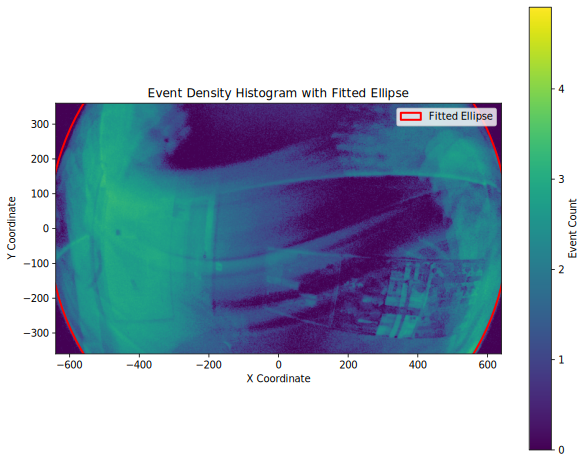
\includegraphics[width=0.7\textwidth]{./fig/svg/ellipse_fit.pdf}
	\caption{Fitted ellipse to the calibration data, with major axis $a = 652$, and minor axis $b = 650$.}
	\label{fig:ellipse_fit}
\end{figure}

Finally, to visualize the calibration results, we map every point from the image plane using the \texttt{cam2world}\footnote{\url{https://github.com/jakarto3d/py-OCamCalib/blob/main/src/pyocamcalib/modelling/camera.py}}
function from py-OCamCalib, which takes a 2D image point, and returns
the corresponding 3D optical ray on the camera's unit sphere. For each point we calculate its angle from the optical axis (a vector $\mathbf{v} = \begin{bmatrix} 0 & 0 & 1 \end{bmatrix}^{T}$),
and mask out the visible area with the ellipse fitted in \reffig{fig:ellipse_fit}. We can see the results in \reffig{fig:calibration_viz}.

\begin{figure}[H]
	\centering
	\includegraphics[width=1.0\textwidth]{./fig/pgfplot/evk4_viz.pdf}
	\caption{Angle from optical axis visualization, with the maximum angle of 93.47 degrees.}
	\label{fig:calibration_viz}
\end{figure}

We can also apply a perspective conversion to the whole image, which now represents distances and angles correctly. We can notice that by looking
at the calibration lattice at \reffig{fig:calib_c}, which now looks like a grid of points.

\begin{figure}[H]
	\centering
	\subfloat[Uncalibrated image.] {
	  \includegraphics[width=0.5\textwidth]{./fig/pgfplot/image_uncalib.pdf}
	  \label{fig:calib_c_1}
	}
	\subfloat[Calibrated image.] {
	  \includegraphics[width=0.5\textwidth]{./fig/pgfplot/image_calib.pdf}
	  \label{fig:calib_c_2}
	}
	\caption{
		Two photos of the calibration lattice, one uncalibrated on \reffig{fig:calib_c_1} and the one calibrated at \reffig{fig:calib_c_2}, which does not
		exhibit any distortion.
  }
	\label{fig:calib_c}
\end{figure}

%% --------------------------------------------------------------
%% |                            RSSR                            |
%% --------------------------------------------------------------

%!TEX root = ../main.tex

\chapter{RSSR\label{chap:rssr}}

TODO: WRITE THIS



%% --------------------------------------------------------------
%% |                            ROS                             |
%% --------------------------------------------------------------

%!TEX root = ../main.tex

\chapter{ROS implementation\label{chap:rssr}}

TODO: WRITE THIS

TODO: DO EXPERIMENT

%% --------------------------------------------------------------
%% |                         Conclusion                         |
%% --------------------------------------------------------------

%!TEX root = ../main.tex

\chapter{Conclusion\label{chap:conclusion}}

This work has shown the influence of distance and frequency of modulated light sources on the response of an event based camera.
We have shown that the average number of events decreases with the increase of distance and can be approximated with
the inverse square law. The average number of events also decreases with the increase of frequency, as the camera is not
able to capture all the changes generated by the light source. What is also possible to observe from the results is the relatively
small distance range, in which the camera detects higher frequencies.

The influence of the rotation angle has also been examined, and has shown that the light source of each of the UAV arms can be
approximated with a lambertian emission model. Each of the arms can then be approximated as two lambertian sources, shifted
by $\pm 45$ degrees from the center of the arm. The real emission pattern approaches the theoretical model with the increase
of distance.

The RSSR method will be used in the subsequent bachelor thesis, where the UAV uses all of its 4 arms with different frequencies
to localize itself in the environment. This will be done by measuring the ratio of the received light intensity from each of the
arms. The camera will need to be calibrated using a calibrattion lattice of LEDs, the video data will need to be morphed
to get rid of the fish eye lens effect and to measure distances correctly.

%% --------------------------------------------------------------
%% |                         References                         |
%% --------------------------------------------------------------

\chapter{References}

\printbibliography[heading=none,title={}]

%% --------------------------------------------------------------
%% |                         Appendices                         |
%% --------------------------------------------------------------

\appendix
\renewcommand\chaptername{Appendix}

\renewcommand{\thechapter}{A}
\renewcommand\chaptername{Appendix A}

\chapter{Appendix A}

\end{document}
